\documentclass{article}

\title{Take Me Out to (Analyze) the Ballgame \\ Visualization and Analysis Techniques for Big Spatial Data}
\author{Chris Comiskey}
\date{\today}

\usepackage{natbib}
\bibliographystyle{unsrtnat}

\usepackage{fullpage}
\usepackage{ulem}
\usepackage{amsmath, amsthm, amssymb, amsfonts}
\usepackage{mathtools}
\usepackage{float}
\usepackage{bbm}
\usepackage{wrapfig}
\usepackage{listings}
\usepackage[utf8]{inputenc}
\usepackage[english]{babel}
\usepackage[export]{adjustbox}

\makeatletter
\def\verbatim@font{\linespread{1}\normalfont\ttfamily}
\makeatother

\usepackage[toc,page]{appendix}


% \setlength{\parindent}{4em}
% \setlength{\parskip}{1em}
% \renewcommand{\baselinestretch}{1.3}

\usepackage{setspace}
\doublespacing

% TESTING =====
\usepackage[T1]{fontenc}
\usepackage[font=small,labelfont=bf,tableposition=top]{caption}
\DeclareCaptionLabelFormat{andtable}{#1~#2  \&  \tablename~\thetable}
% TESTING =====


\begin{document}
\maketitle{}

\tableofcontents


\section{Introduction} % ================================================

\subsection{``Get a Good Ball to Hit''}
In 1971 left-handed hitter Ted Williams published what many baseball players consider a bible of their craft,``The Science of Hitting'' \citep{Williams1971}. In it Williams credits another baseball legend, Rogers Hornsby, as giving him the best piece of advice he ever received: ``Get a good ball to hit.''
        \begin{figure}[H]
      	\centering
      	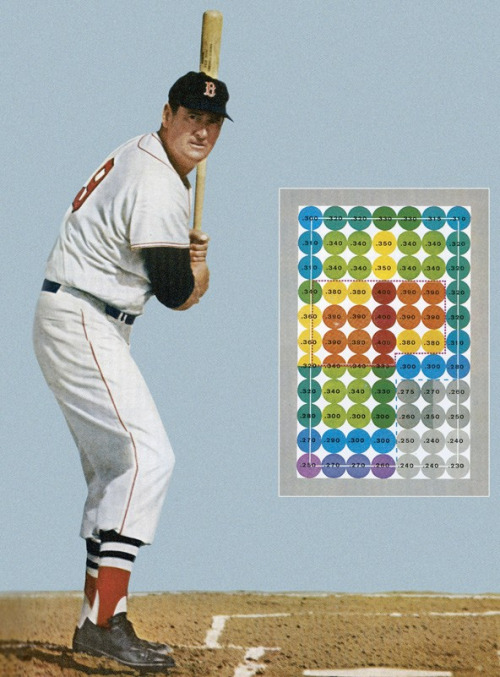
\includegraphics[scale=.29]{Images/Williams.jpg} 
      	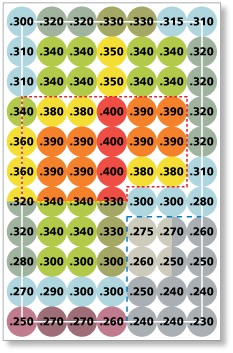
\includegraphics[scale=0.55]{Images/SZ.jpg}
      	\caption{Ted Williams conceptualized of the strike zone as divided into locations for pitches on which he would have specific probabilities of getting a hit. In this iconic image he labeled the baseballs with his own estimated batting average on pitches in that location \citep{Williams1971}.}
      	\end{figure} 
Horsby meant that location makes some pitches easier to hit than others, and  Williams's famous strike zone image, shown in Figure 1, visualizes this advice\footnote{For background information on the rules and workings of the game of baseball, please see Appendix A, or \citep{Wiki}}. Until 2008, data did not exist to explore, visualize, and model William's location-based conceptualization of the stike zone. However, in 2008 MLB collaborated with Sportsvision, to implement a new technology called PITCHf/x\textsuperscript{\textregistered}, and began collecting the necessary data.


\subsection{The Data} % ============================================
Sportvision, Inc., a company based in Chicago, provides the technology to collect PITCHf/x\textsuperscript{\textregistered} data. In 2007 and 2008 Sportvision installed two high speed stereoscopic cameras in every MLB\textsuperscript{\textregistered} stadium. These cameras take 20 images of each pitch in flight and determine its 3-D path \citep{Fast2010}. Sportsvision licenses the collected PITCHf/x\textsuperscript{\textregistered} data to Major League Baseball Advanced Media (MLBAM\textsuperscript{\textregistered}) \citep{Baumer2010}. MLBAM\textsuperscript{\textregistered} provides the PITCHf/x\textsuperscript{\textregistered} data to the public in XML format as part of  their  `Gameday' data, at their website \citep{Sievert2014}. A homepage exists for every game, with links organizing data into XML tables such as game, inning, at bat, pitch, team, player, umpire, etc. \citep{Sievert2014}. The at bat table, for example, contains 15 variables for 1,711,211 at bats. The format and size (on the order of gigabytes) of the data makes a manual download impractical. Instead, XML downloading scripts are advised to create a database \citep{Adler2006}. We used the MySQL database management system  to manipulate and store 13 PITCHf/x\textsuperscript{\textregistered} tables \citep{Tahaghoghi2006}. Data of this size requires finessing R's ``memory management'' \citep{Wickham2014}. This is because R is an ``{\it in-memory} application,'' which means a computer's limited RAM hosts the R environment data \citep{Smith2013}. To avoid overwhelming R's working memory limitations, we applied the Split-Apply-Combine strategy to tables inside the MySQL database before importing data frames to R \citep{Wickham2011}.

We collected the variables relevant for this research predominantly from the `at bat' and `pitches' tables. These variables, with a short description, are the following \citep{Fast2007}.
  \begin{itemize}
  \item \verb|px| - location of the pitch on the horizontal axis when it passes through the strike zone (or the extended plane). \verb|px| is recorded in feet from the middle of home plate, from the catcher/umpire point of view.
  \item \verb|pz| - location of the pitch on the vertical axis when it passes through the strike zone plane, measured in feet above the ground. A negative value implies the ball bounced before reaching home plate
  \item \verb|des| - a short description of the outcome of the pitch, i.e. swing and miss, ground ball for out, ground ball for hit, etc.  
  \item \verb|id| - a unique id for a pitch within a game
  \item \verb|ab_id| - a unique id for each at bat  
  \item \verb|pitch_id| - a unique identification number for each pitch
  \item \verb|pitch_type| - a classification of the type of pitch, out of 18 possible types. For example, four seam fastball, two seam fastball, curveball, knuckle ball, etc.
  \item \verb|stand| - handedness of the batter; right or left.
  \item \verb|batter| - a unique ID for each hitter
  \end{itemize}

% The variable \verb|des|, short for `description,' describes pitch outcomes. In this study, we use swing outcomes described in \verb|des| to define a Bernoulli random variable $S$ (Section 3.1) that equals one for a hit, and equals zero for {\it any} swing that does not result in a hit. This modifies the current standard, where analyses include only swings that end at bats \citep{Cross2015}, \citep{Baumer2010}, \citep{Fast2011}. We submit that {\it every} swing represents a trial, and failure to get a hit should be evaluated separately from the count in the at bat at the time of the trial.

\subsection{Practical Significance of Data Analysis in Baseball}

Major League Baseball (MLB\textsuperscript{\textregistered}) teams exploy approximately 156 quantitative analysts, at a total cost of approximately \$15 million annually \citep{Lindbergh2016}. Teams strive to gain marginal competitive advantages, so novel modeling and analysis of strike zone data could generate substantial interest. For example, results indicate hitters have higher success probabilities in the lower 1/3 of the strike zone than in the top 1/3, but this contradicts conventional wisdom advising pitchers to ``keep the ball down'' \citep{Stallings2003}. An interpretable model that explains why this is bad advice may change minds. As a second example, if these interpretations are in biomechanical language, biomechanists may analyze the relationships between body types and spatial success probabilities. This could in turn help MLB\textsuperscript{\textregistered} team scouting departments more accurately preduct hitting success for amateur players, a notorously difficult but lucrative challenge. For a final example, some MLB\textsuperscript{\textregistered} players, such as Joey Votto, have a keen interest in using the most sophisticated analytics available to understand the keys to their success and failure\citep{Daugherty2015}. This research would fit that criteria for Votto.

With regard to media usage possibilities, heat maps are frequently included in television broadcasts of MLB\textsuperscript{\textregistered} games \citep{Cross2015}. ESPN\textsuperscript{\textregistered} and MLB\textsuperscript{\textregistered} recently agreed to an eight year, \$5.6 billion contract \citep{Newman2012}; cutting-edge, more informative heat maps would improve the quality of game broadcasts.

As the dollar amounts indicate, it is not for a lack of motivation that the research questions posed here remain open. Rather, the solutions require an array of statistical and computational competencies. In addition, the data are quite new, and relatively inaccessible without data management and programming skills.

% The methods we will use for addressing these questions will include and integrate generalized linear models \citep{Myers2012}, spatial statistics \citep{Oliver2005}, and Bayesian hierarchical models \citep{Gelman2014}. We will employ these methodologies using the statistical software R \citep{R2015}, the Bayesian statistical software and programming language Stan \citep{Gelman2015}, the R to Stan interface RStan \citep{RSTAN}, advanced data visualization tools in ggplot2 \citep{Wickham2009}, baseball specific programming techniques \citep{Marchi2013}, and the open-source Relational Database Management System (RDMS) MySQL \citep{Tahaghoghi2006} for storing and managing a 1.82 GB (to date) PITCHf/x\textsuperscript{\textregistered} database.

\subsection{Research Roadmap}

% Using PITCHf/x\textsuperscript{\textregistered} data, amateur statisticians have conducted exploratory data analysis of the spatial, hitter success, strike zone data. However, there have been virtually no publicly available\footnote{Presumably proprietary approaches by MLB\textsuperscript{\textregistered} teams exist.} professional or academic attempts to model and understand the spatial process with advanced statistical techniques. 

Chapter 2 uses strike zone data to explore the problem of resolution selection for empirical heat maps with varying spatial data density. We provide a new option for addressing this problem, which we call varying-resolution heat maps. Two parts comprise Chapter 3. In the first part we create a generalized linear model for spatial hitter success probabilities, using biomechanical covariates manufactured from a switch to the polar coordinate system and a strategically translated origin. In the second part we confront the question of how to improve the current approach to presenting heat map confidence intervals. We provide, we believe, a better option with an interactive Shiny application \citep{Shiny}. In Chapter 3 we add a spatial random effect to the Chapter 2 model, and deal with the computational consequences; we define the ``Big N'' problem, and explore three approaches to fitting a ``Big N'' spatial generalized linear mixed model. 


\bibliography{Baseball}

\end{document}